\documentclass[10pt]{article}
\usepackage[utf8]{inputenc}
\usepackage{geometry}
\usepackage[sort]{natbib}
\usepackage{pxfonts}
\usepackage{graphicx}
% \graphicspath{ {./figures-low/} }
\graphicspath{ {./figures-default/} }
\usepackage{setspace}
\usepackage{hyperref}
\usepackage{lineno}
\usepackage{authblk}
\usepackage{pdflscape}
\usepackage{rotating}
\usepackage{multirow}
\usepackage[online,flushleft]{threeparttable}
\usepackage{booktabs}

\doublespacing
\linenumbers

\title{\textit{Supplementary materials for:} The psychological arrow of time drives temporal asymmetries in inferring unobserved past and future events}
\author[1]{Xinming Xu}
\author[2]{Ziyan Zhu}
\author[3]{Xueyao Zheng}
\author[1, $\star$]{Jeremy R. Manning}
\affil[1]{Dartmouth College, Hanover, NH, USA}
\affil[2]{Peking University, Beijing, China}
\affil[3]{Beijing Normal University, Beijing, China}
\affil[$\star$]{Address correspondence to jeremy.r.manning@dartmouth.edu}

% figures from the main text
\newcommand{\intro}{1}
\newcommand{\methods}{2}
\newcommand{\resultOne}{3}
\newcommand{\resultTwo}{4}
\newcommand{\resultThree}{5}
\newcommand{\resultFour}{6}
\newcommand{\resultFive}{7}
\newcommand{\metaAnalysis}{8}
\newcommand{\discussion}{9}

\begin{document}
\maketitle

\renewcommand{\thefigure}{S\arabic{figure}}
\renewcommand{\thetable}{S\arabic{table}}


\begin{table}[]
\caption{\textbf{Stimulus descriptions (main experiment).}}
\begin{center}
\resizebox{\textwidth}{!}{
\begin{threeparttable}
\begin{tabular}{rrrrlll}
\toprule
\multirow{2}{*}{Storyline} &
  \multirow{2}{*}{Segment} &
  \multirow{2}{*}{Episode} &
  \multirow{2}{*}{Duration (s)} &
  \multirow{2}{*}{Main characters} &
  \multicolumn{2}{l}{Number of events\tnote{a}} \\ \cmidrule(l){6-7} 
  &    &   &     &                                & Onscreen      & Offscreen\tnote{b} \\ \midrule
1 & 1  & 1 & 105 & Beth, Sheila, Rob, Leo         & 4             & 7         \\
1 & 2  & 1 & 172 & Beth, Sheila, Rob, Leo         & 7 {[}1{]}     & 3         \\
1 & 3  & 1 & 70  & Beth, Sheila, One neighbor     & 6             & 2         \\
1 & 4  & 1 & 135 & Beth, Sheila                   & 8 {[}1{]}     & 1         \\
1 & 5  & 1 & 90  & Beth, Rob, April               & 8             & 4         \\
1 & 6  & 1 & 188 & Beth, Rob                      & 6 {[}2{]}     & 1         \\
1 & 7  & 1 & 91  & Beth, Sheila                   & 5 {[}1{]}     & 2         \\
1 & 8  & 1 & 142 & Beth, April                    & 4 (1) {[}2{]} & 3 (1)     \\
1 & 9  & 2 & 134 & Beth, April                    & 4 {[}2{]}     & 1         \\
1 & 10 & 2 & 58  & Beth                           & 3 {[}1{]}     & 6 {[}1{]} \\
1 & 11 & 2 & 159 & Beth, Rob                      & 9             &           \\
2 & 1  & 1 & 70  & Simone, Karl                   & 3 {[}1{]}     & 6         \\
2 & 2  & 1 & 119 & Simone, Karl, Naomi, Tommy     & 4 {[}1{]}     & 2         \\
2 & 3  & 1 & 58  & Simone, Karl, Tommy            & 4             & 2         \\
2 & 4  & 1 & 102 & Simone, Karl                   & 4             & 6         \\
2 & 5  & 1 & 134 & Simone, Karl, Tommy            & 6 (3) {[}1{]} & 3         \\
2 & 6  & 1 & 81  & Simone, Karl, Neighbors, Wanda & 4 (1)         & 6         \\
2 & 7  & 1 & 194 & Simone, Tommy                  & 8             & 3         \\
2 & 8  & 2 & 101 & Simone, Karl                   & 3 (1)         & 1         \\
2 & 9  & 2 & 86  & Simone, Tommy                  & 4 {[}1{]}     & 3         \\
2 & 10 & 2 & 232 & Simone, Karl                   & 6 {[}1{]}     & 3         \\
2 & 11 & 2 & 189 & Simone, Naomi, Tommy           & 7 (1) {[}1{]} &           \\ \bottomrule
\end{tabular}
\begin{tablenotes}
\item[a] Number of partial events (see methods) shown in parentheses; number of summary events shown in square brackets.
\item[b] Offscreen events happened between the current segment and the next segment.
\end{tablenotes}
\end{threeparttable}
}
\end{center}
\end{table}


\begin{table}[]
\caption{\textbf{Stimulus descriptions (replication experiment).}}
\begin{center}
\resizebox{\textwidth}{!}{
\begin{threeparttable}
\begin{tabular}{rrlll}
\toprule
\multirow{2}{*}{Segment} &
  \multirow{2}{*}{Duration (s)} &
  \multirow{2}{*}{Main characters} &
  \multicolumn{2}{l}{Number of events\tnote{a}} \\ \cmidrule(l){4-5} 
 &     &                                & Onscreen      & Offscreen\tnote{b} \\ \midrule
1 & 258 & Ji-Yoon, All faculty; Bill, Doodles\tnote{c}         & 14 (1) [1]      & 1        \\
2 & 40 & Joan, All faculty         & 3 (2)    & 0         \\
3 & 87  & Dean, Ji-Yoon      & 7 [1]          & 3         \\
4 & 78 & Elliot, Yasmine           & 5 [1]  & 1         \\
5 & 66  & Ji-Yoon, Yasmine           & 2 [1]             & 9 (1)         \\
6 & 212 & Bill; Bill, Dafna; Elliot, Yasmine        & 11 (2)    & 1         \\
7 & 134  & Ji-Yoon, Joan                & 5 (3)    & 0         \\
8 & 38 & Bill, Lila                & 2 & 0     \\
9 & 35 & Elliot, Yasmine                   & 1    & 2 (1)         \\
10 & 164  & Bill, Ji-Yoon                           & 8 [2]     & 5 \\
11 & 154 & Ji-Yoon, Habi, JuJu                     & 5 [1]             &   9 [1]        \\
12 & 216  & Joan; Ji-Yoon, Lila; Ji-Yoon, Bill         & 6 [1]     & 0         \\
13 & 56 & Ji-Yoon, Bill          & 2 [1] &           \\ \bottomrule
\end{tabular}
\begin{tablenotes}
\item[a] Number of partial events (see methods) shown in parentheses; number of summary events shown in square brackets.
\item[b] Offscreen events happened between the current segment and the next segment.
\item[c] Characters from different scenes are separated by ";".
\end{tablenotes}
\end{threeparttable}
}
\end{center}
\end{table}


\begin{table}
    \footnotesize
    \caption{List of datasets analyzed in our meta-analysis (see Fig. 8).}
    \label{tab:datasets}
    \begin{tabular}{p{0.6in}|l|p{2.2in}|l|p{0.5in}|p{0.5in}|p{0.5in}}
        \toprule
        \textbf{Dataset} & \textbf{Short name} & \textbf{Description} & \textbf{Category} & \textbf{Number of observations} & \textbf{Ob\-ser\-va\-tion type} & \textbf{Number of words} \\
        \midrule
        Internet Movie Script Database & IMSDb & A collection of transcripts from roughly 1000 popular movies. & Film & 1091 & Transcript & 26023348 \\
        \midrule
        Movie Dialogues Dataset & Movies & A large collection of fictional conversations extracted from raw movie scripts. & Film & 304713 & Utterance & 3209921 \\
        \midrule
        Switchboard Dialog Act Corpus & Switchboard & A collection of five-minute telephone conversations between two participants, annotated with speech act tags. & Speech & 122646 & Utterance & 2052779 \\
        \midrule
        Supreme Court Corpus & SCOTUS & A collection of cases from the U.S. Supreme Court, along with transcripts of oral arguments. & Speech & 1700789 & Utterance & 71889094 \\
        \midrule
        Tennis Interviews & Tennis & Transcripts for tennis singles post-match press conferences for major tournaments between 2007 to 2015. & Speech & 163948 & Utterance & 7043118 \\
        \midrule
        Persuasion for Good Corpus & PfG & A collection of online conversations generated by Amazon Mechanical Turk workers, where one participant (the persuader) tries to convince the other (the persuadee) to donate to a charity. & Speech & 20932 & Utterance & 351759 \\
        \midrule
        Intelligence Squared Debates Corpus & IQ2 & This dataset contains transcripts of debates held as part of Intelligence Squared Debates. & Speech & 26562 & Utterance & 1898509 \\
        \midrule
        Group Affect and Performance Corpus & GAP & Group members completed a Winter Survival Task (WST), a group decision-making exercise where participants must rank 15 items according to their importance in a hypothetical plane crash scenario. Participants first rank the items individually. Then, each group was given a maximum of 15 minutes to complete the WST. The group’s conversations and deliberations during this task were recorded as conversations in this dataset. & Speech & 8009 & Utterance & 45989 \\
        \midrule
        The Chair & Chair & Scraped transcripts from The Chair, Season 1. & Television & 6 & Transcript & 19197 \\
        \midrule
        Friends Corpus & Friends & A collection of all the conversations that occurred over 10 seasons of Friends, a popular American TV sitcom that ran in the 1990s. & Television & 67373 & Utterance & 622894 \\
        \midrule
        Gutenberg Dialogue Dataset & Gutenberg & Dialogues extracted from the Project Gutenberg collection. & Text & 14773741 & Utterance & 327519461 \\
        \midrule
        Reddit Corpus & Reddit & A collection of Corpuses of Reddit data built from Pushshift.io Reddit Corpus. Each Corpus contains posts and comments from an individual subreddit from its inception until Oct 2018. & Text & 74468 & Utterance & 3080662 \\
        \bottomrule
    \end{tabular}
\end{table}




\begin{table}
    \footnotesize
    \centering

    \caption{Part of speech pattern templates used to identify verb tenses in
    our meta analysis. Part of speech tags are represented between angled
    brackets, and pipes ($|$) denote instances where \textit{any} of the two or
    more parts of speech are considered a match when they appear at the given
    position in the indicated sequence. The plus signs ($+$) denote that one or
    more repetitions of the given sequence within a single sentence are still
    counted as a ``single'' instance of the given tense. Part of speech tags
    are defined in Table~\ref{tab:pos_tags}.}

    \begin{tabular}{r|l}
    \toprule
      \textbf{Tense} & \textbf{Pattern template} \\
      \midrule
      conditional continuous & $<$MD$>$$<$BE$>$$<$VBG$|$HVG$|$BEG$>$$+$ \\
      \midrule
      conditional continuous passive & $<$MD$>$$<$BE$>$$<$BEG$>$$<$VBN$|$VBD$>$$+$ \\
      \midrule
      conditional indefinite & $<$MD$>$$<$BE$|$DO$|$VB$|$HV$>$$+$ \\
      \midrule
      conditional indefinite passive & $<$MD$>$$<$BE$>$$<$VBN$|$VBD$>$$+$ \\
      \midrule
      conditional perfect & $<$MD$>$$<$HV$>$$<$HVN$|$BEN$|$VBN$|$VBD$>$$+$ \\
      \midrule
      conditional perfect continuous & $<$MD$>$$<$HV$>$$<$BEN$>$$<$VBG$|$HVG$|$BEG$>$$+$ \\
      \midrule
      conditional perfect passive & $<$MD$>$$<$HV$>$$<$BEN$>$$<$VBN$|$VBD$>$$+$ \\
      \midrule
      future continuous & $<$MDF$>$$<$BE$>$$<$VBG$|$HVG$|$BEG$>$$+$ \\
      \midrule
      future continuous passive & $<$MDF$>$$<$BE$>$$<$BEG$>$$<$VBN$|$VBD$>$$+$ \\
      \midrule
      future indefinite & $<$MDF$>$$<$BE$|$DO$|$VB$|$HV$>$$+$ \\
      \midrule
      future indefinite passive & $<$MDF$>$$<$BE$>$$<$VBN$|$VBD$>$$+$ \\
      \midrule
      future perfect & $<$MDF$>$$<$HV$>$$<$HVN$|$BEN$|$VBN$|$VBD$>$$+$ \\
      \midrule
      future perfect continuous & $<$MDF$>$$<$HV$>$$<$BEN$>$$<$VBG$|$HVG$|$BEG$>$$+$ \\
      \midrule
      future perfect continuous passive & $<$MDF$>$$<$HV$>$$<$BEN$>$$<$BEG$>$$<$VBN$|$VBD$>$$+$ \\
      \midrule
      future perfect passive & $<$MDF$>$$<$HV$>$$<$BEN$>$$<$VBN$|$VBD$>$$+$ \\
      \midrule
      infinitive & $<$TO$>$$<$BE$|$HV$|$VB$>$$+$ \\
      \midrule
      past continuous & $<$BED$|$BEDZ$>$$<$VBG$|$HVG$|$BEG$>$$+$ \\
      \midrule
      past continuous passive & $<$BED$|$BEDZ$>$$<$BEG$>$$<$VBN$|$VBD$>$$+$ \\
      \midrule
      past indefinite & $<$DOD$>$$<$VB$|$HV$|$DO$>$$|$$<$BEDZ$|$BED$|$HVD$|$VBN$|$VBD$>$$+$ \\
      \midrule
      past indefinite passive & $<$BED$|$BEDZ$>$$<$VBN$|$VBD$>$$+$ \\
      \midrule
      past perfect & $<$HVD$>$$<$BEN$|$VBN$|$HVD$|$HVN$>$$+$ \\
      \midrule
      past perfect continuous & $<$HVD$>$$<$BEN$>$$<$HVG$|$BEG$|$VBG$>$$+$ \\
      \midrule
      past perfect continuous passive & $<$HVD$>$$<$BEN$>$$<$BEG$>$$<$VBN$|$VBD$>$$+$ \\
      \midrule
      past perfect passive & $<$HVD$>$$<$BEN$>$$<$VBN$|$VBD$>$$+$ \\
      \midrule
      present continuous & $<$BEM$|$BER$|$BEZ$>$$<$BEG$|$VBG$|$HVG$>$$+$ \\
      \midrule
      present continuous passive & $<$BEM$|$BER$|$BEZ$>$$<$BEG$>$$<$VBN$|$VBD$>$$+$ \\
      \midrule
      present indefinite & $<$DO$|$DOZ$>$$<$DO$|$HV$|$VB$>$$+$$|$$<$DO$|$HV$|$VB$|$BEZ$|$DOZ$|$BER$|$HVZ$|$BEM$|$VBZ$>$$+$ \\
      \midrule
      present indefinite passive & $<$BEM$|$BER$|$BEZ$>$$<$VBN$|$VBD$>$$+$ \\
      \midrule
      present perfect & $<$HV$|$HVZ$>$$<$BEN$|$HVD$|$VBN$|$VBD$>$$+$ \\
      \midrule
      present perfect continuous & $<$HV$|$HVZ$>$$<$BEN$>$$<$VBG$|$BEG$|$HVG$>$$+$ \\
      \midrule
      present perfect continuous passive & $<$HV$|$HVZ$>$$<$BEN$>$$<$BEG$>$$<$VBN$|$VBD$>$$+$ \\
      \midrule
      present perfect passive & $<$HV$|$HVZ$>$$<$BEN$>$$<$VBN$|$VBD$>$$+$ \\
      \bottomrule
    \end{tabular}
    \label{tab:regexp_templates}
\end{table}


\begin{table}[h!]
    \centering
    \caption{Part of speech tag definitions.}
    \begin{tabular}{r|l}
        \toprule
        \textbf{Tag} & \textbf{Part of speech} \\
        \midrule
        BE & Be \\
        \midrule
        BEG & Related to beginning or gerundive form \\
        \midrule
        BEM & Am (first person singular present of BE) \\
        \midrule
        BEN & Been (past participle of BE) \\
        \midrule
        BER & Are (second person singular and all plural present of BE) \\
        \midrule
        BEZ & Is (third person singular present of BE) \\
        \midrule
        BED & Were (past plural of BE) \\
        \midrule
        BEDZ & Was (past singular of BE) \\
        \midrule
        DO & Do \\
        \midrule
        DOD & Did (past tense of DO) \\
        \midrule
        DOZ & Do, 3rd person singular present \\
        \midrule
        HV & Have (archaic form for historical texts) \\
        \midrule
        HVD & Have, past tense (archaic) \\
        \midrule
        HVG & Have, gerund or present participle (archaic) \\
        \midrule
        HVN & Have, past participle (archaic) \\
        \midrule
        HVZ & Have, 3rd person singular present (archaic) \\
        \midrule
        MD & Modal \\
        \midrule
        MDF & Modal, future tense \\
        \midrule
        TO & To \\
        \midrule
        VB & Verb, base form \\
        \midrule
        VBD & Verb, past tense \\
        \midrule
        VBG & Verb, gerund or present participle \\
        \midrule
        VBN & Verb, past participle \\
        \midrule
        VBP & Verb, non-3rd person singular present \\
        \midrule
        VBZ & Verb, 3rd person singular present \\
        \bottomrule
    \end{tabular}
    \label{tab:pos_tags}
  \end{table}

  \begin{table}[h!]
    \centering
    \caption{Keywords and phrases used to identify references to the past.}
    \begin{tabular}{l l l l l}
    \toprule
    ago & elapsed & last month & olden days & thus far \\
    \midrule
    already & expired & last night & once & to date \\
    \midrule
    antiquity & final & last quarter & once upon a time & up to now \\
    \midrule
    back when & formerly & last season & previously & used to \\
    \midrule
    before & had & last semester & recently & used to be \\
    \midrule
    bygone & heretofore & last time & said & was \\
    \midrule
    ceased & historically & last week & since & were \\
    \midrule
    concluded & hitherto & last year & so far & wrote \\
    \midrule
    did & in the past & long ago & terminated & yesterday \\
    \midrule
    earlier & in those days & made & then & yesteryear \\
    \bottomrule
    \end{tabular}
    \label{tab:keywords_past}
  \end{table}
  
  \begin{table}[h!]
    \centering
    \caption{Keywords and phrases used to identify references to the future.}
    \begin{tabular}{l l l l l}
        \toprule
        after & going to & later & next time & shortly \\
        \midrule
        anticipated & hereafter & later on & next week & some day \\
        \midrule
        can & imminently & looming & next year & soon \\
        \midrule
        could & impending & may & on the horizon & subsequent \\
        \midrule
        down the line & in the cards & might & plan to & succeeding \\
        \midrule
        eventual & in the future & next month & predicted & to be \\
        \midrule
        eventually & in the works & next quarter & prospective & tomorrow \\
        \midrule
        forthcoming & in time & next season & scheduled to & upcoming \\
        \midrule
        futuristic & intend to & next semester & shall & will \\
        \bottomrule
    \end{tabular}
    \label{tab:keywords_future}
  \end{table}

  \newpage


\begin{figure}[tp]
    \centering
    \includegraphics[width=\textwidth]{methods_rep}
      \caption{\textbf{Task overview (replication experiment).} Participants in our replication experiment watched segments from the television series \textit{The Chair}. They made free-form text responses to either retrodict what had happened in the previous segment, or predict what would happen in the next segment. We systematically varied whether participants watched the segments in forward or reverse chronological order, whether (or not) responses were cued using the main characters in the target segment, and which other segments participants had watched prior to making a response. For each segment, we collected several retrodiction or prediction across different experimental conditions. Experiment time is denoted along the vertical axis, storyline segments orders are indicated along the horizontal axis, and the colors denote experimental tasks (conditions).}
    \label{fig:methods_rep}
\end{figure}

\begin{figure}[tp]
    \centering
    \includegraphics[width=\textwidth]{supp1}
    \caption{\textbf{Mean proportion of target events hit (A), precision (B), and convergence (C) as a function of number of segments watched in each storyline, in participants' uncued and character-cued retrodictions and predictions (main experiment).} Grey lines represent the least squares fits.}
    \label{fig:supp1}
\end{figure}

\begin{figure}[tp]
    \centering
    \includegraphics[width=\textwidth]{supp1_rep}
    \caption{\textbf{Mean proportion of target events hit (A), precision (B), and convergence (C) as a function of number of segments watched, in participants' uncued and character-cued retrodictions and predictions (replication experiment).} Grey lines represent the least squares fits.}
    \label{fig:supp1_rep}
\end{figure}

\begin{figure}[tp]
    \centering
    \includegraphics[width=\textwidth]{supp2}
    \caption{\textbf{Mean number of events hit for each event type, in participants' uncued and character-cued retrodictions and predictions, averaged across just-watched segments (main experiment).}}
    \label{fig:supp2}
\end{figure}

\begin{figure}[tp]
    \centering
    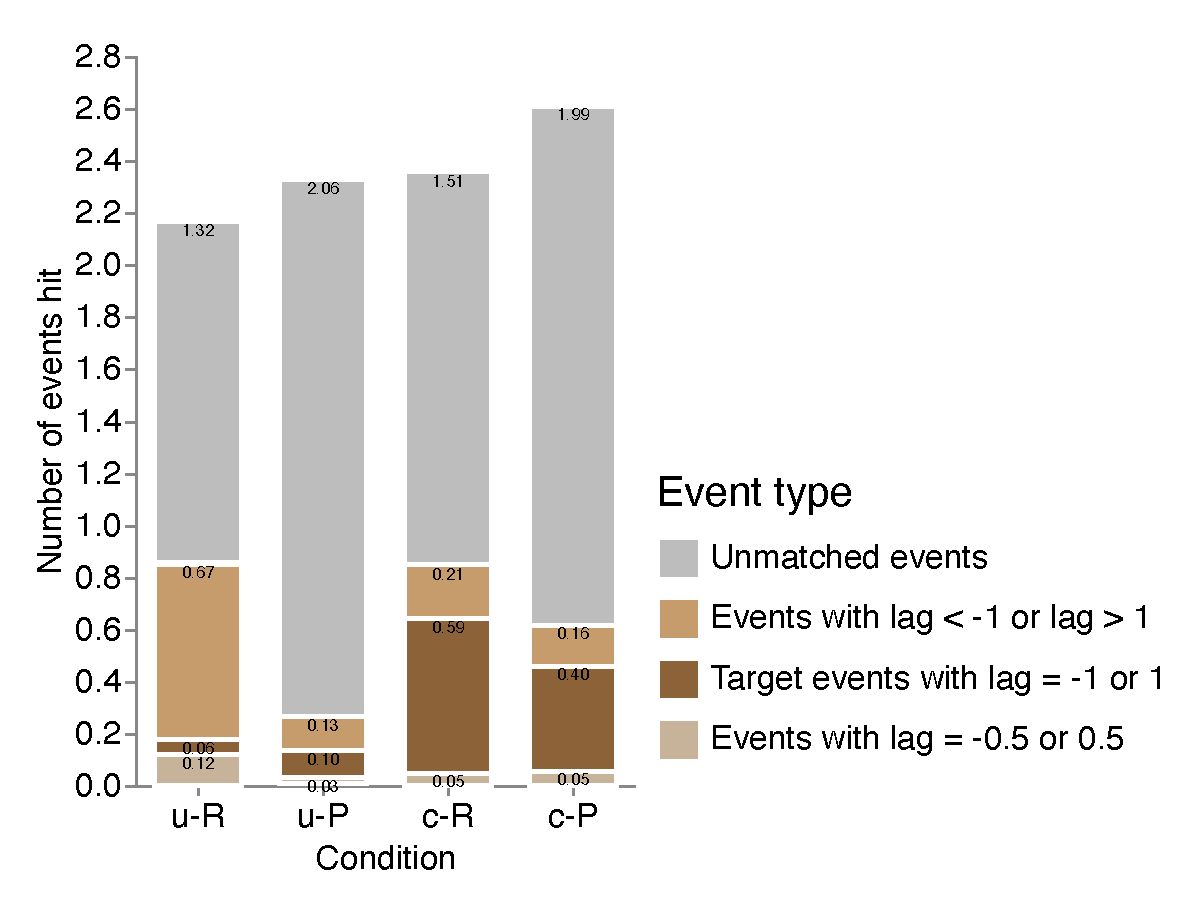
\includegraphics[width=\textwidth]{supp2_rep}
    \caption{\textbf{Mean number of events hit for each event type, in participants' uncued and character-cued retrodictions and predictions, averaged across just-watched segments (replication experiment).}}
    \label{fig:supp2_rep}
\end{figure}

\begin{figure}[tp]
    \centering
    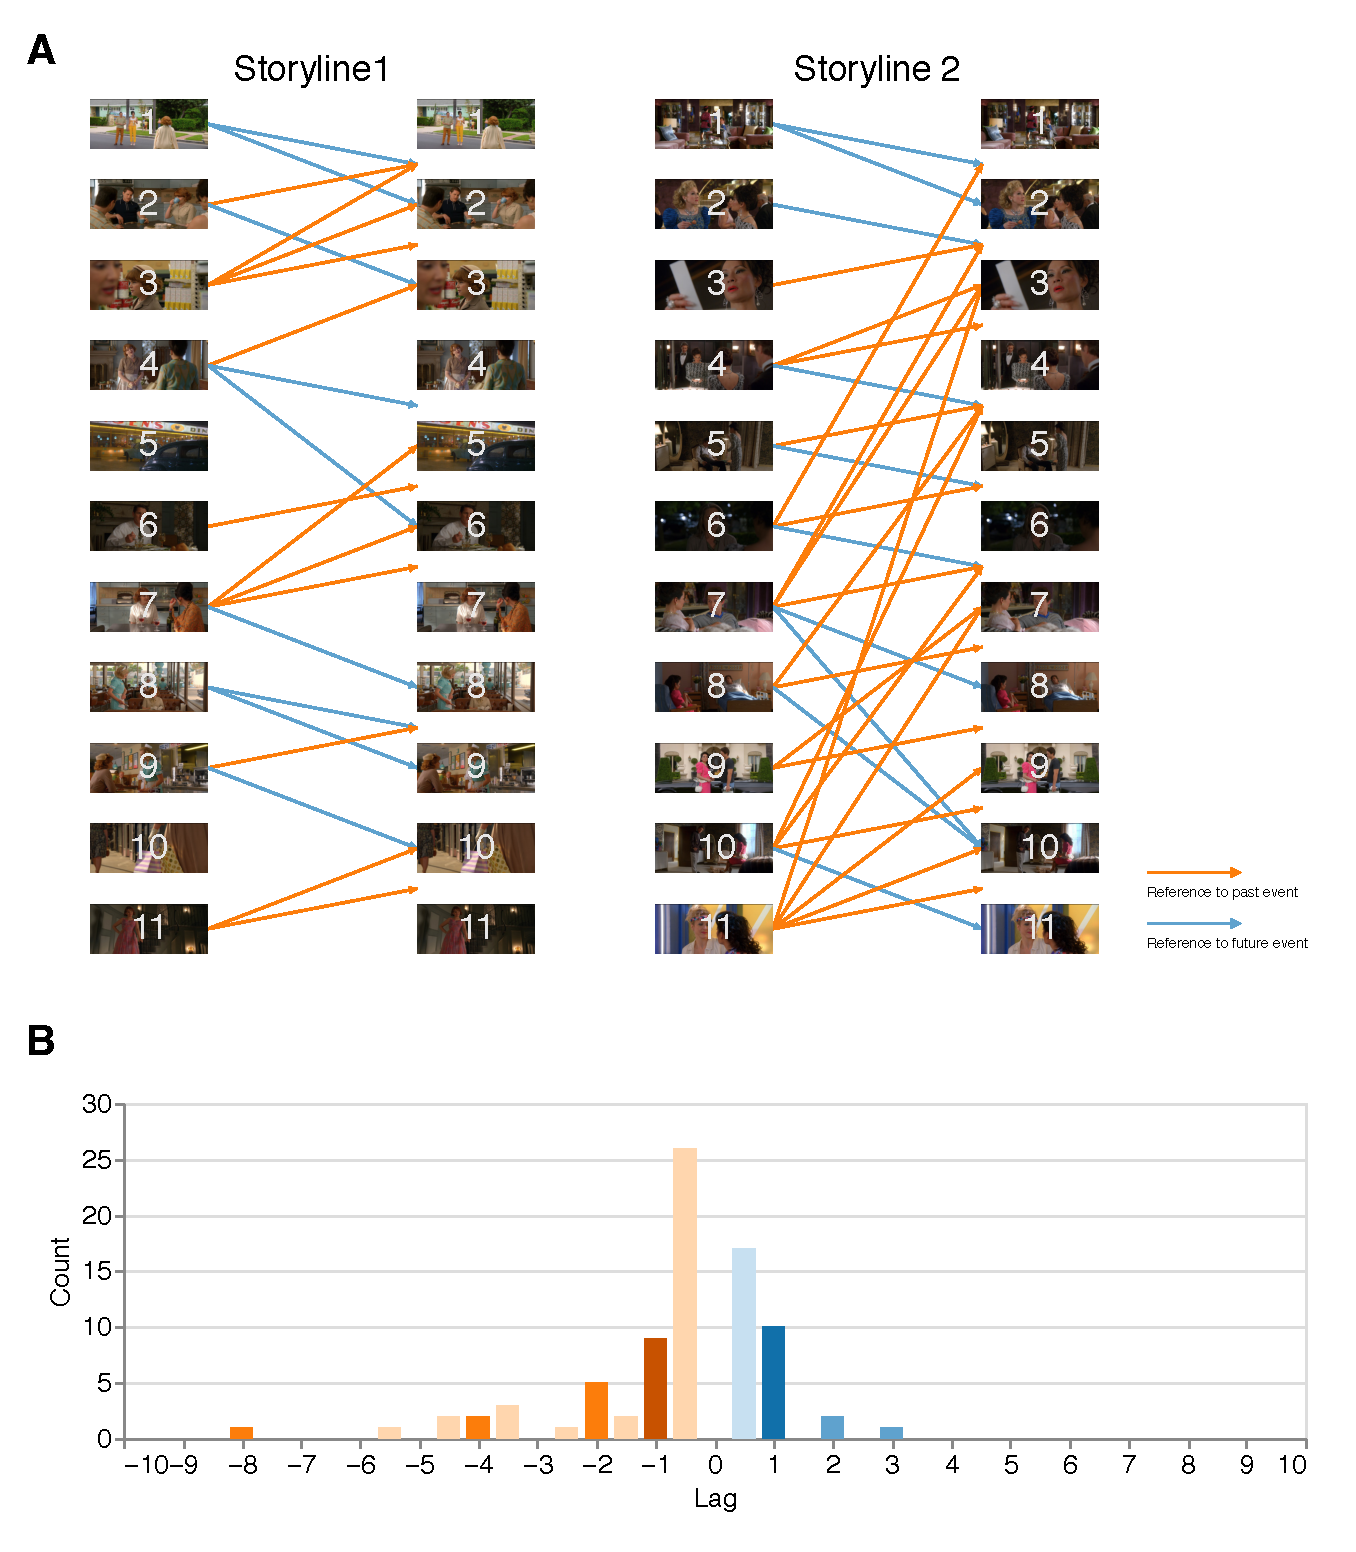
\includegraphics[width=\textwidth]{supp3}
    \caption{\textbf{(A)} All references in each storyline (main experiment). \textbf{(B)} Distribution of reference lags (main experiment).}
    \label{fig:supp3}
\end{figure}

\begin{figure}[tp]
    \centering
    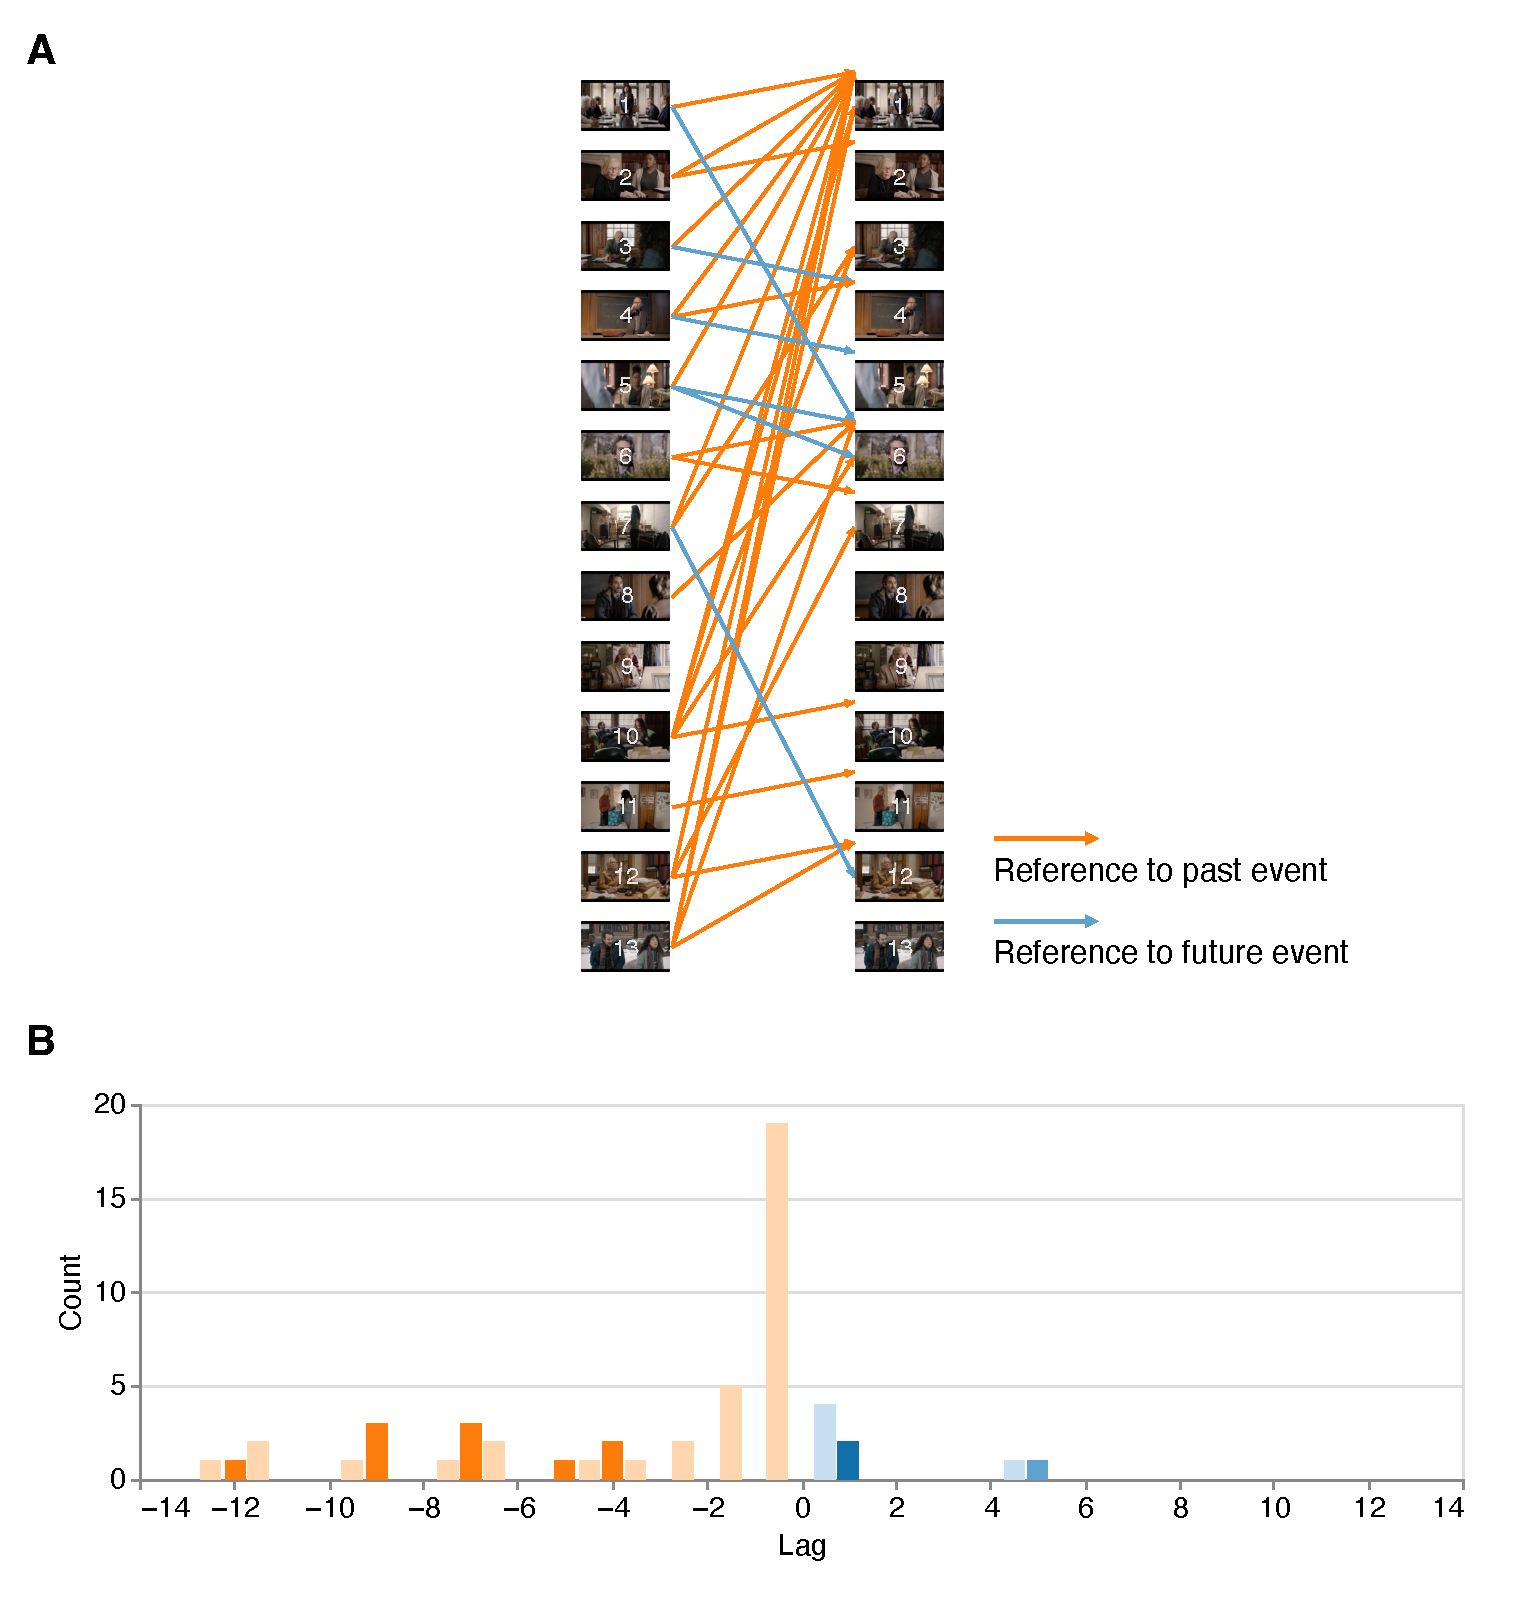
\includegraphics[width=\textwidth]{supp3_rep}
    \caption{\textbf{(A)} All references (replication experiment). \textbf{(B)} Distribution of reference lags (replication experiment).}
    \label{fig:supp3_rep}
\end{figure}

\begin{figure}[tp]
    \centering
    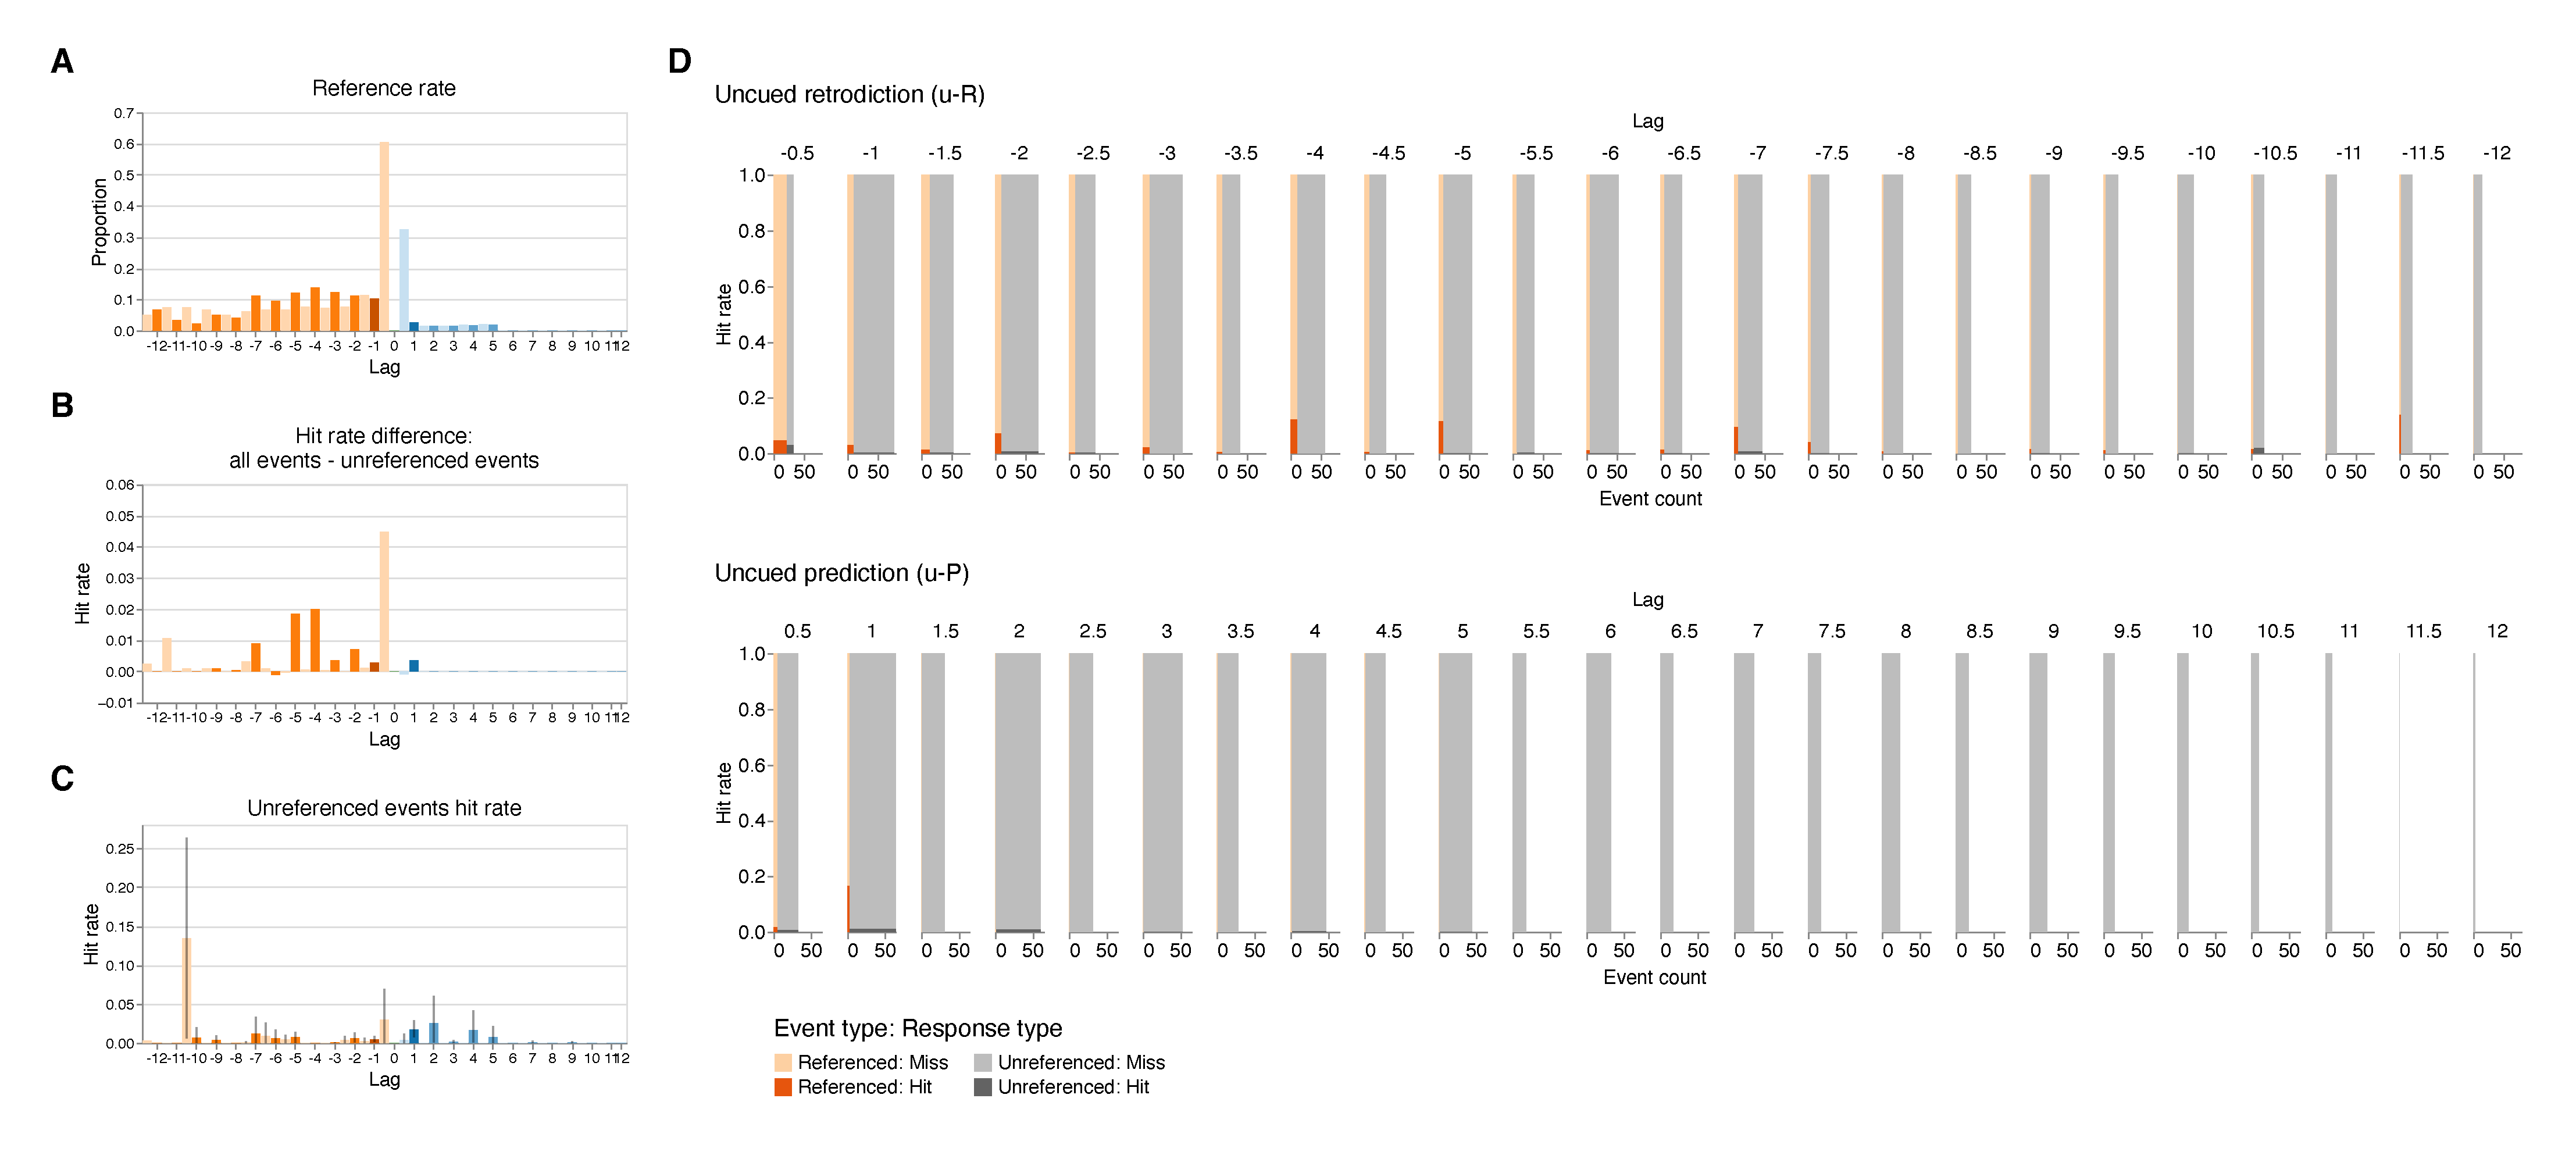
\includegraphics[width=\textwidth]{results3_rep}

      \caption{\textbf{Characters' references drive participants' retrodiction performance (replication experiment).} \textbf{A. Reference rate as a function of lag.} Across all possible just-watched segments (lag 0), the bar heights denote the average proportions of events referenced in other past or future segments. \textbf{B. Difference in hit rates between all events and unreferenced events.} To highlight the effect of characters' references to past and future events on participants' retrodictions and predictions, here we display the difference in across-segment mean hit rates between all events and unreferenced events, as a function of temporal distance (lag) to the just-watched segment. \textbf{C. Hit rates for unreferenced events.} The average response hit rates for unreferenced events are displayed as a function of temporal distance to the just-watched segment. Error bars denote bootstrapped 95\% confidence intervals. Panels A--C: colors are described in the Figure~\resultTwo~caption. \textbf{D. Hit rates and counts of referenced and unreferenced events.} As a function of temporal distance to the just-watched segment, the sub-panels display the across-segment mean numbers ($x$-axes) and hit rates ($y$-axes) of referenced (red) and unreferenced (gray) events that participants hit (darker shading) or missed (lighter shading) in their uncued retrodictions (top sub-panel) and uncued predictions (bottom sub-panel). Intuitively, the widths of the rectangles at each lag denote the total number of events at each possible lag. The darker shading denotes the proportions of events that participants retrodicted or predicted, and the lighter shading denotes the proportions of events that participants ``missed'' in their responses.}
      
    \label{fig:result3_rep}
\end{figure}

\begin{figure}[tp]
    \centering
    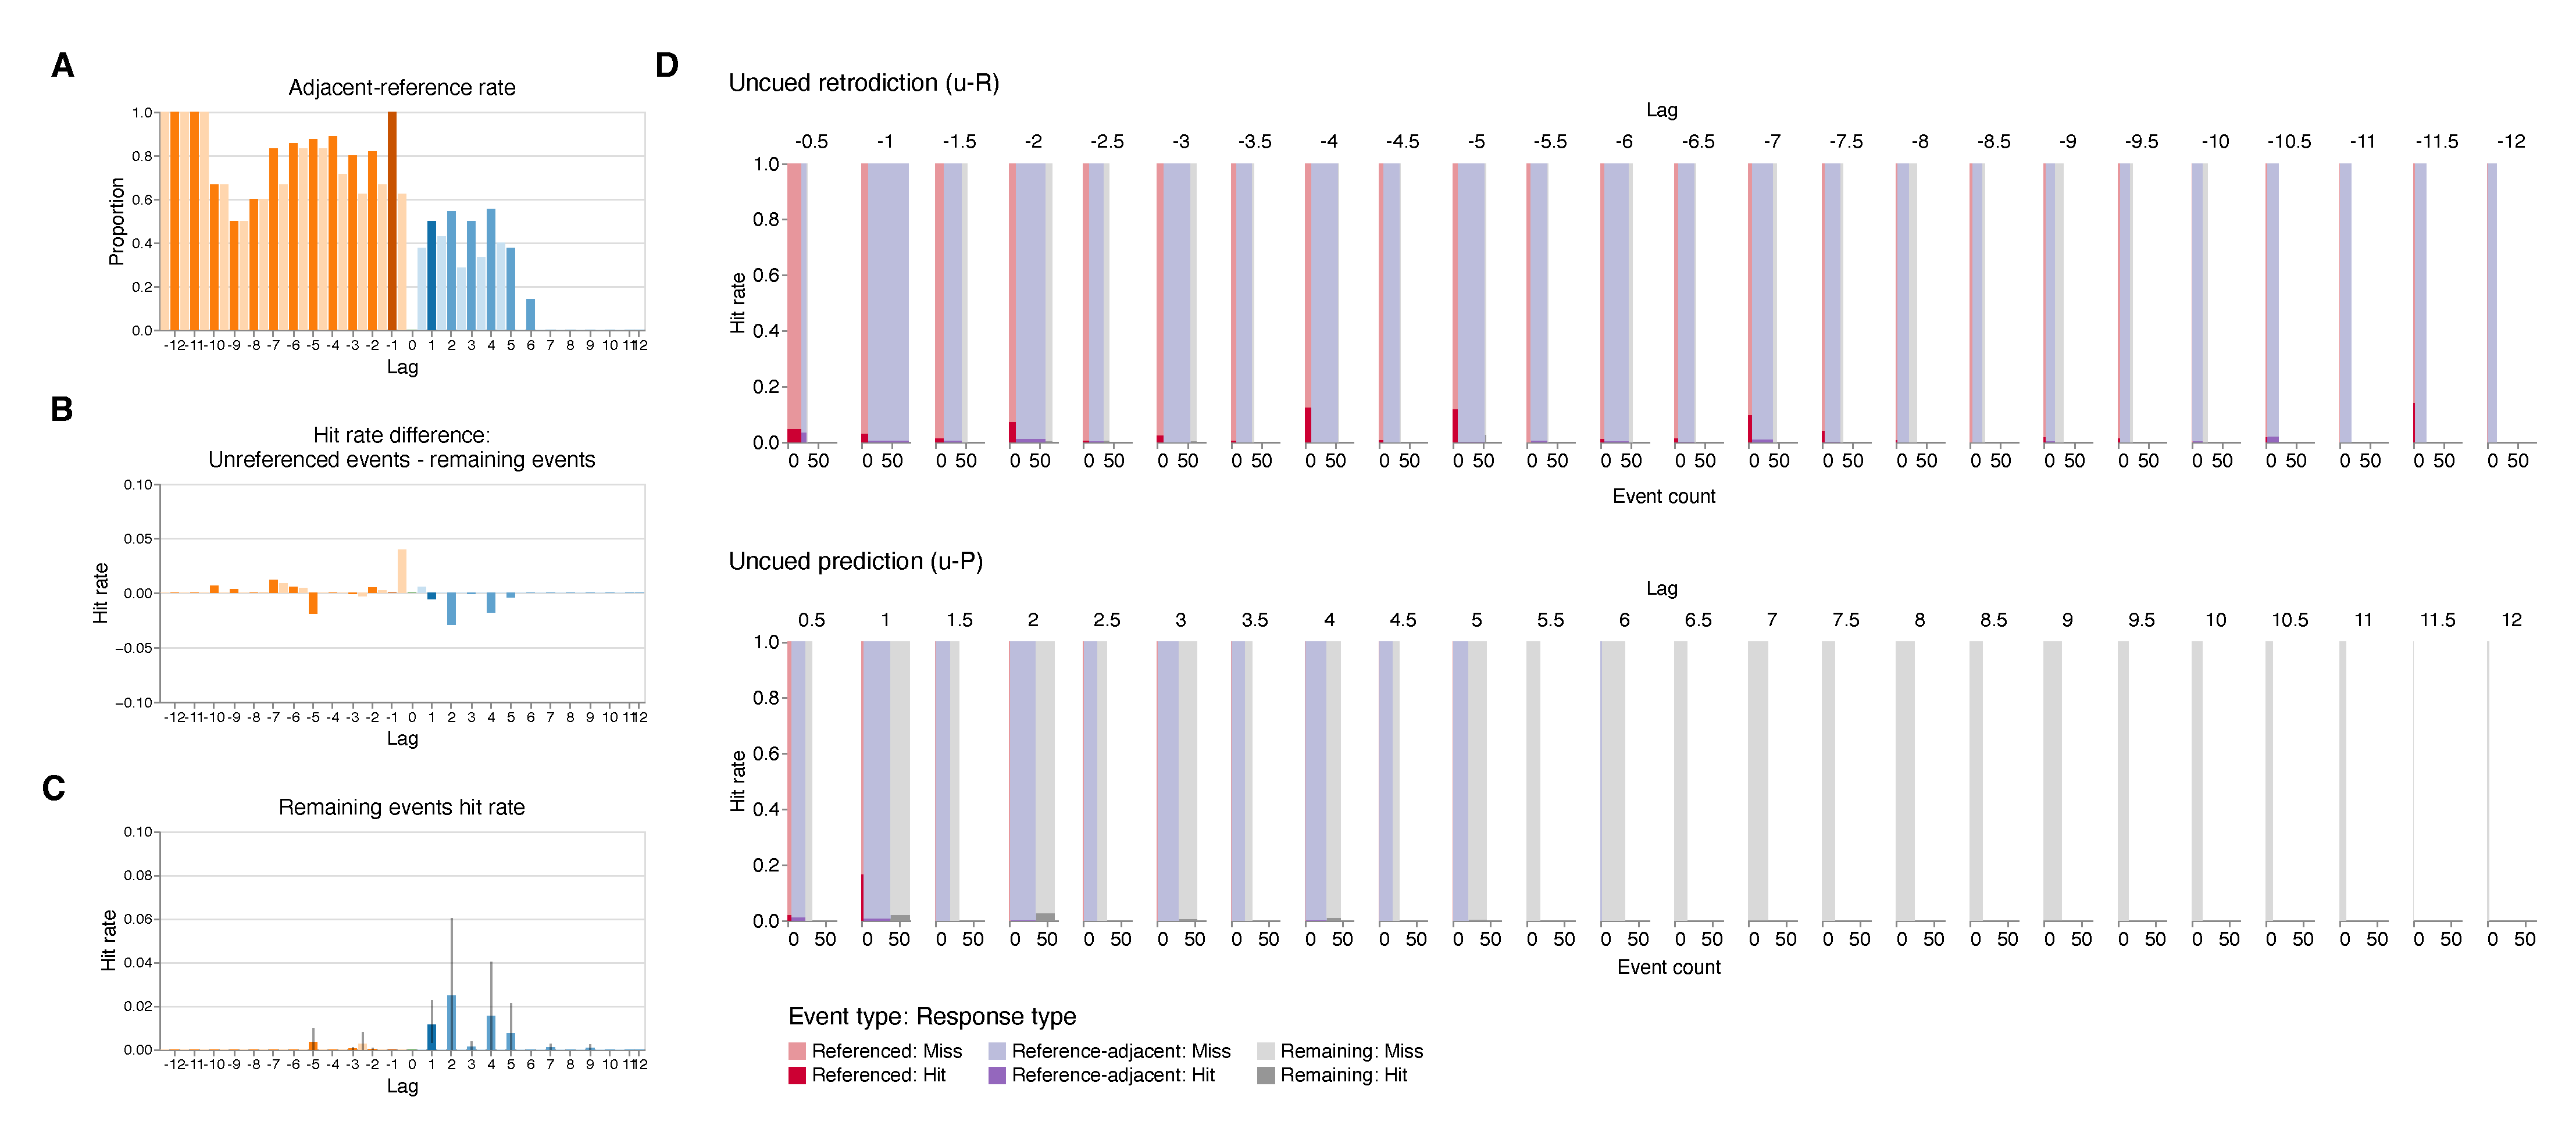
\includegraphics[width=\textwidth]{results4_rep_ori}
      
        \caption{\textbf{Hit rates of reference-adjacenet events (replication experiment).} \textbf{A. Adjacent reference rate for unreferenced events as a function of lag.} Across all possible just-watched segments (lag 0), the bar heights denote the average proportion of unreferenced events in other past or future segments that were temporally adjacent to any referenced event. \textbf{B. Difference in hit rates between unreferenced events and remaining events.} To highlight the effect of reference adjacency on retrodiction and prediction of unreferenced events, here we display the difference in across-segment mean hit rates between unreferenced events and remaining events, as a function of temporal distance (lag) to the just-watched segment. \textbf{C. Hit rates for remaining events.} The across-segment mean response hit rates for unreferenced events that were \textit{not} temporally adjacent to any referenced events are displayed as a function of temporal distance to the just-watched segment. Error bars denote bootstrapped 95\% confidence intervals. Panels A--C: colors are described in the Figure~\resultTwo~caption. \textbf{D. Hit rates and counts of referenced, reference-adjacent, and remaining events.} As a function of temporal distance to the just-watched segment, the sub-panels display the numbers ($x$-axes) and proportions ($y$-axes) of referenced (red), reference-adjacent (purple), and remaining (gray) events that participants hit (darker shading) or missed (lighter shading) in their uncued retrodictions (top sub-panel) and uncued predictions (bottom sub-panel).}
        
    \label{fig:result4_rep_ori}
\end{figure}

\begin{figure}[tp]
    \centering
    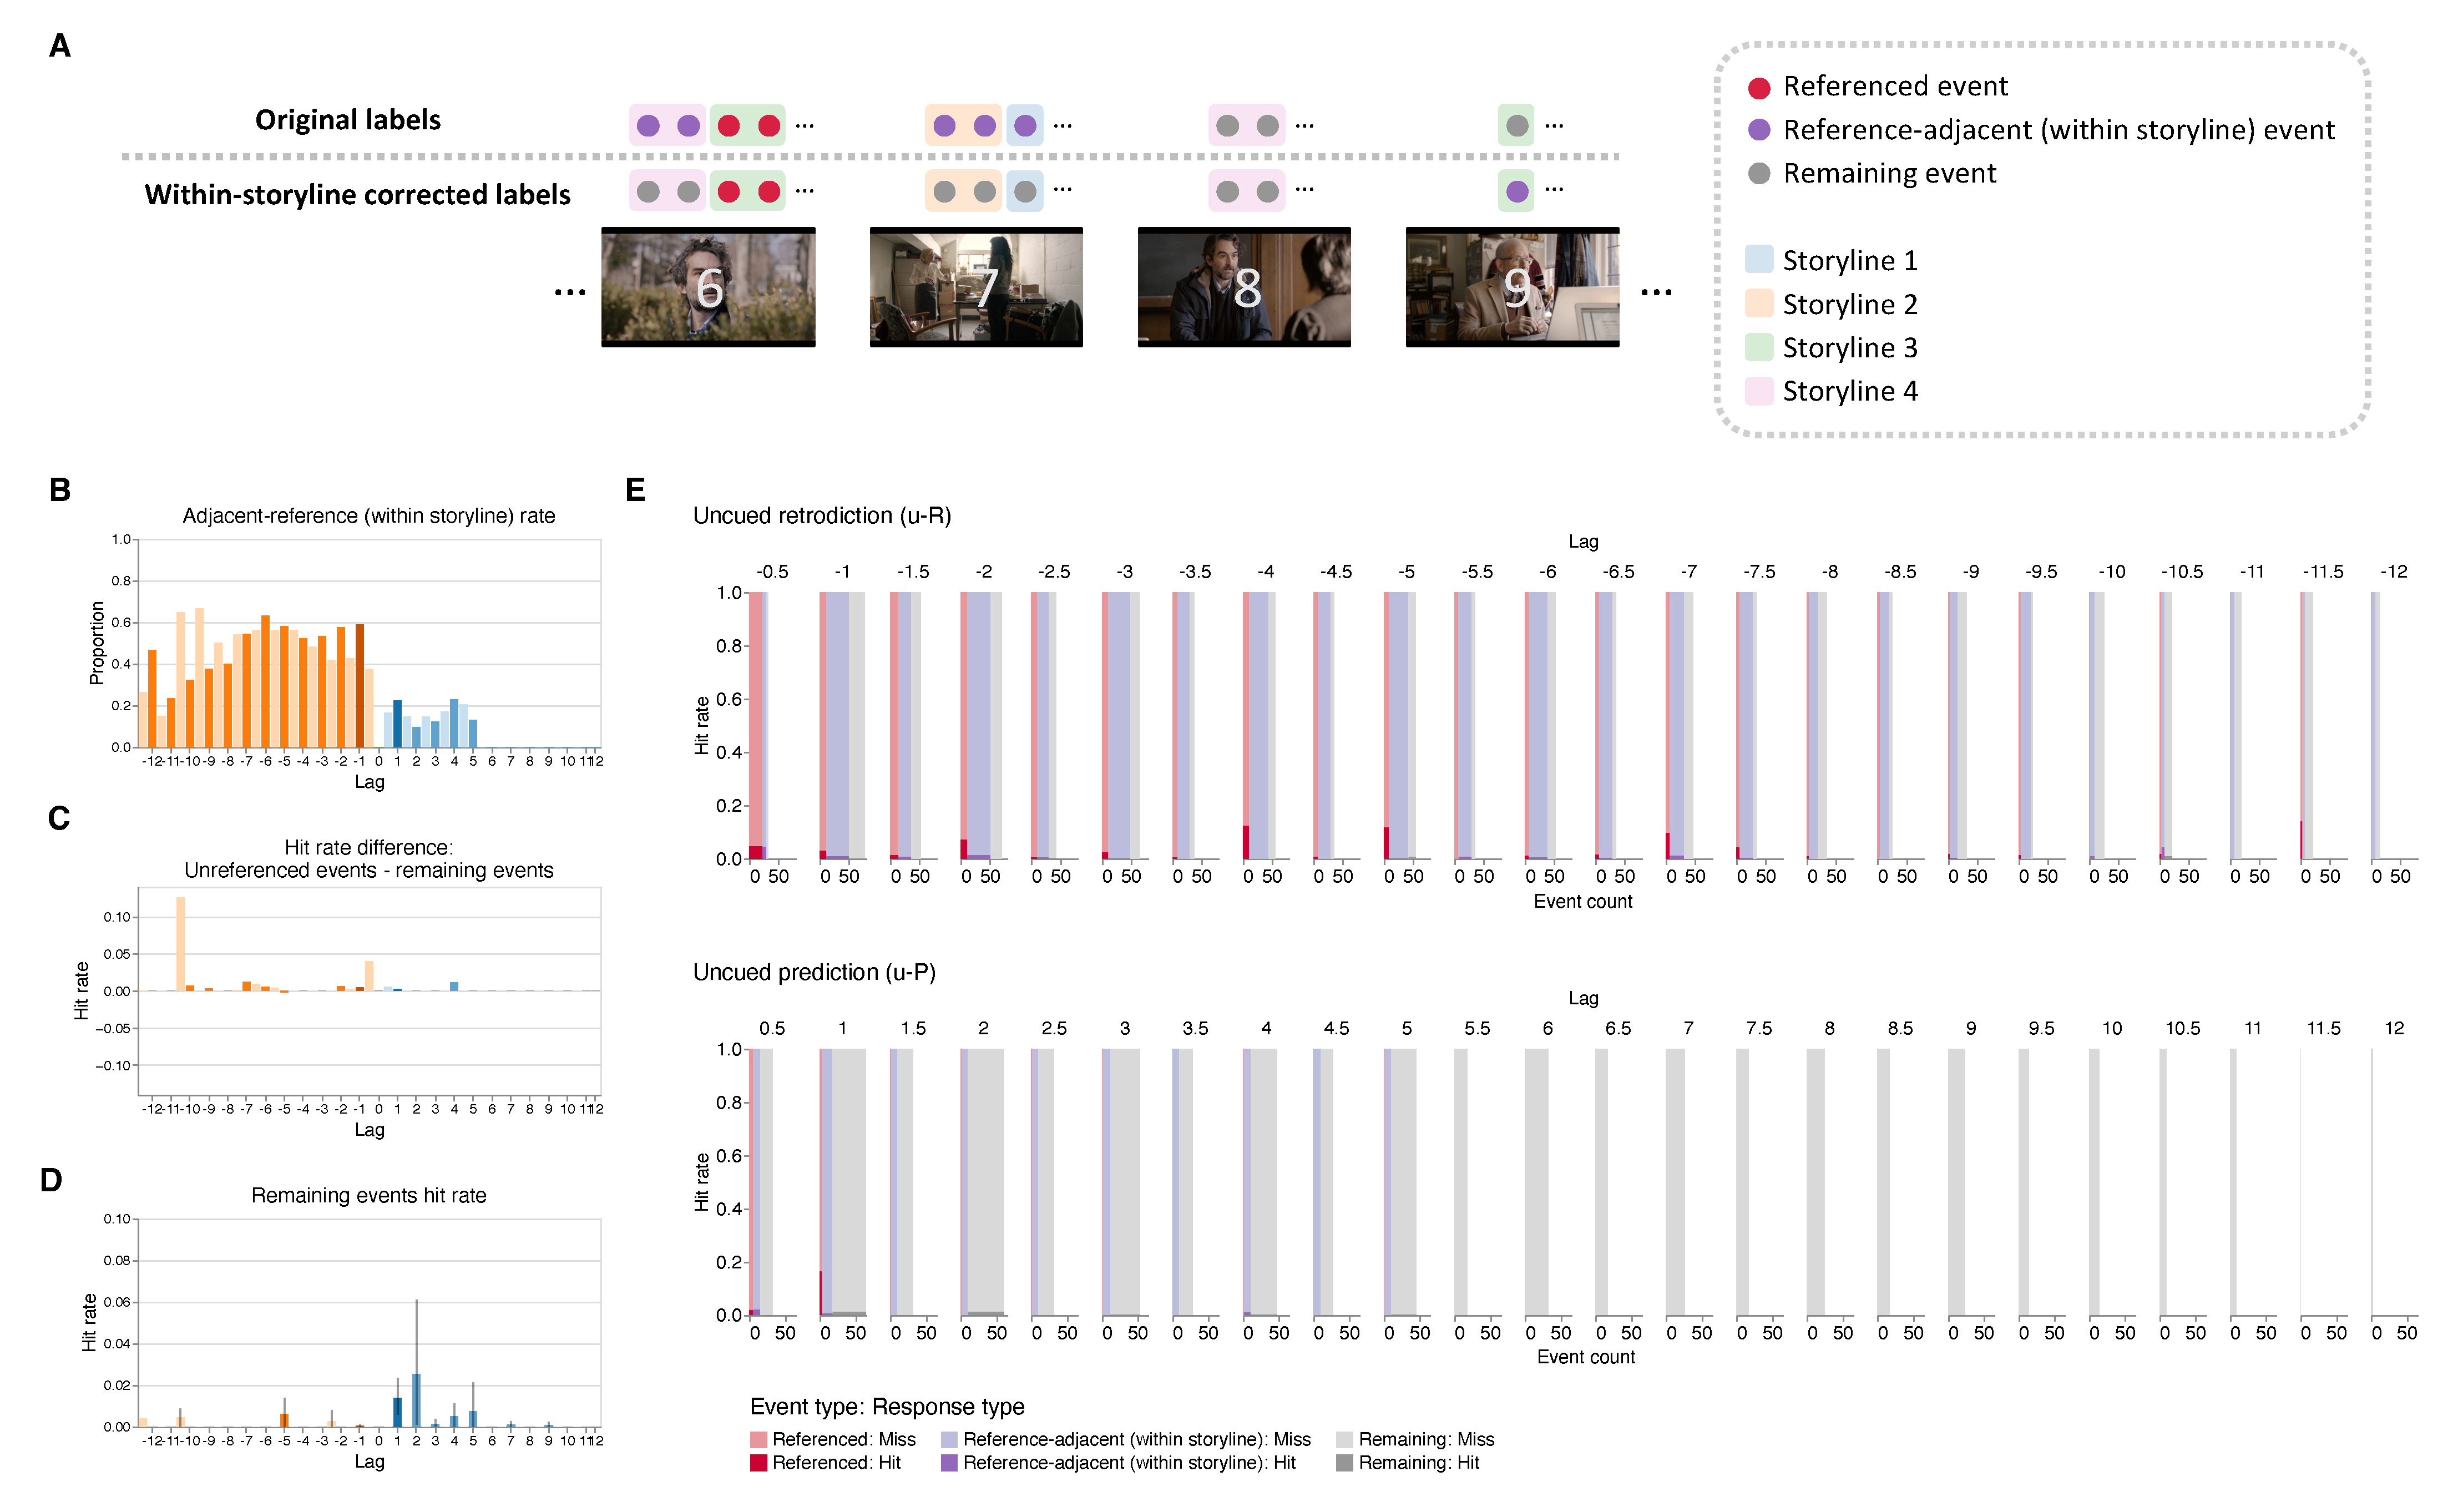
\includegraphics[width=\textwidth]{results4_rep_sl}
    
      \caption{\textbf{Within-storyline reference-adjacent events are associated with higher hit rates (replication experiment).} \textbf{A. Illustration of annotation approach.} Rather than labeling reference-adjacent events as whether they were temporally adjacent to a referenced event using the original segment sequences, here we used within-storyline corrected reference-adjacency labels. We determined four storylines in the segments used in the replication experiment and assigned a storyline label for each event (shown as different background colors of each event). We then labeled reference-adjacent events as whether they were temporally adjacent to a referenced event within the same storyline (same background colors). \textbf{B. Adjacent reference rate for unreferenced events as a function of lag.} Across all possible just-watched segments (lag 0), the bar heights denote the average proportion of unreferenced events in other past or future segments that were temporally adjacent to any referenced event. \textbf{C. Difference in hit rates between unreferenced events and remaining events.} To highlight the effect of reference adjacency on retrodiction and prediction of unreferenced events, here we display the difference in across-segment mean hit rates between unreferenced events and remaining events, as a function of temporal distance (lag) to the just-watched segment. \textbf{D. Hit rates for remaining events.} The across-segment mean response hit rates for unreferenced events that were \textit{not} temporally adjacent to any referenced events are displayed as a function of temporal distance to the just-watched segment. Error bars denote bootstrapped 95\% confidence intervals. Panels A--C: colors are described in the Figure~\resultTwo~caption. \textbf{E. Hit rates and counts of referenced, reference-adjacent, and remaining events.} As a function of temporal distance to the just-watched segment, the sub-panels display the numbers ($x$-axes) and proportions ($y$-axes) of referenced (red), reference-adjacent (purple), and remaining (gray) events that participants hit (darker shading) or missed (lighter shading) in their uncued retrodictions (top sub-panel) and uncued predictions (bottom sub-panel).}
      
    \label{fig:results4_rep_sl}
\end{figure}

\begin{figure}[tp]
    \centering
    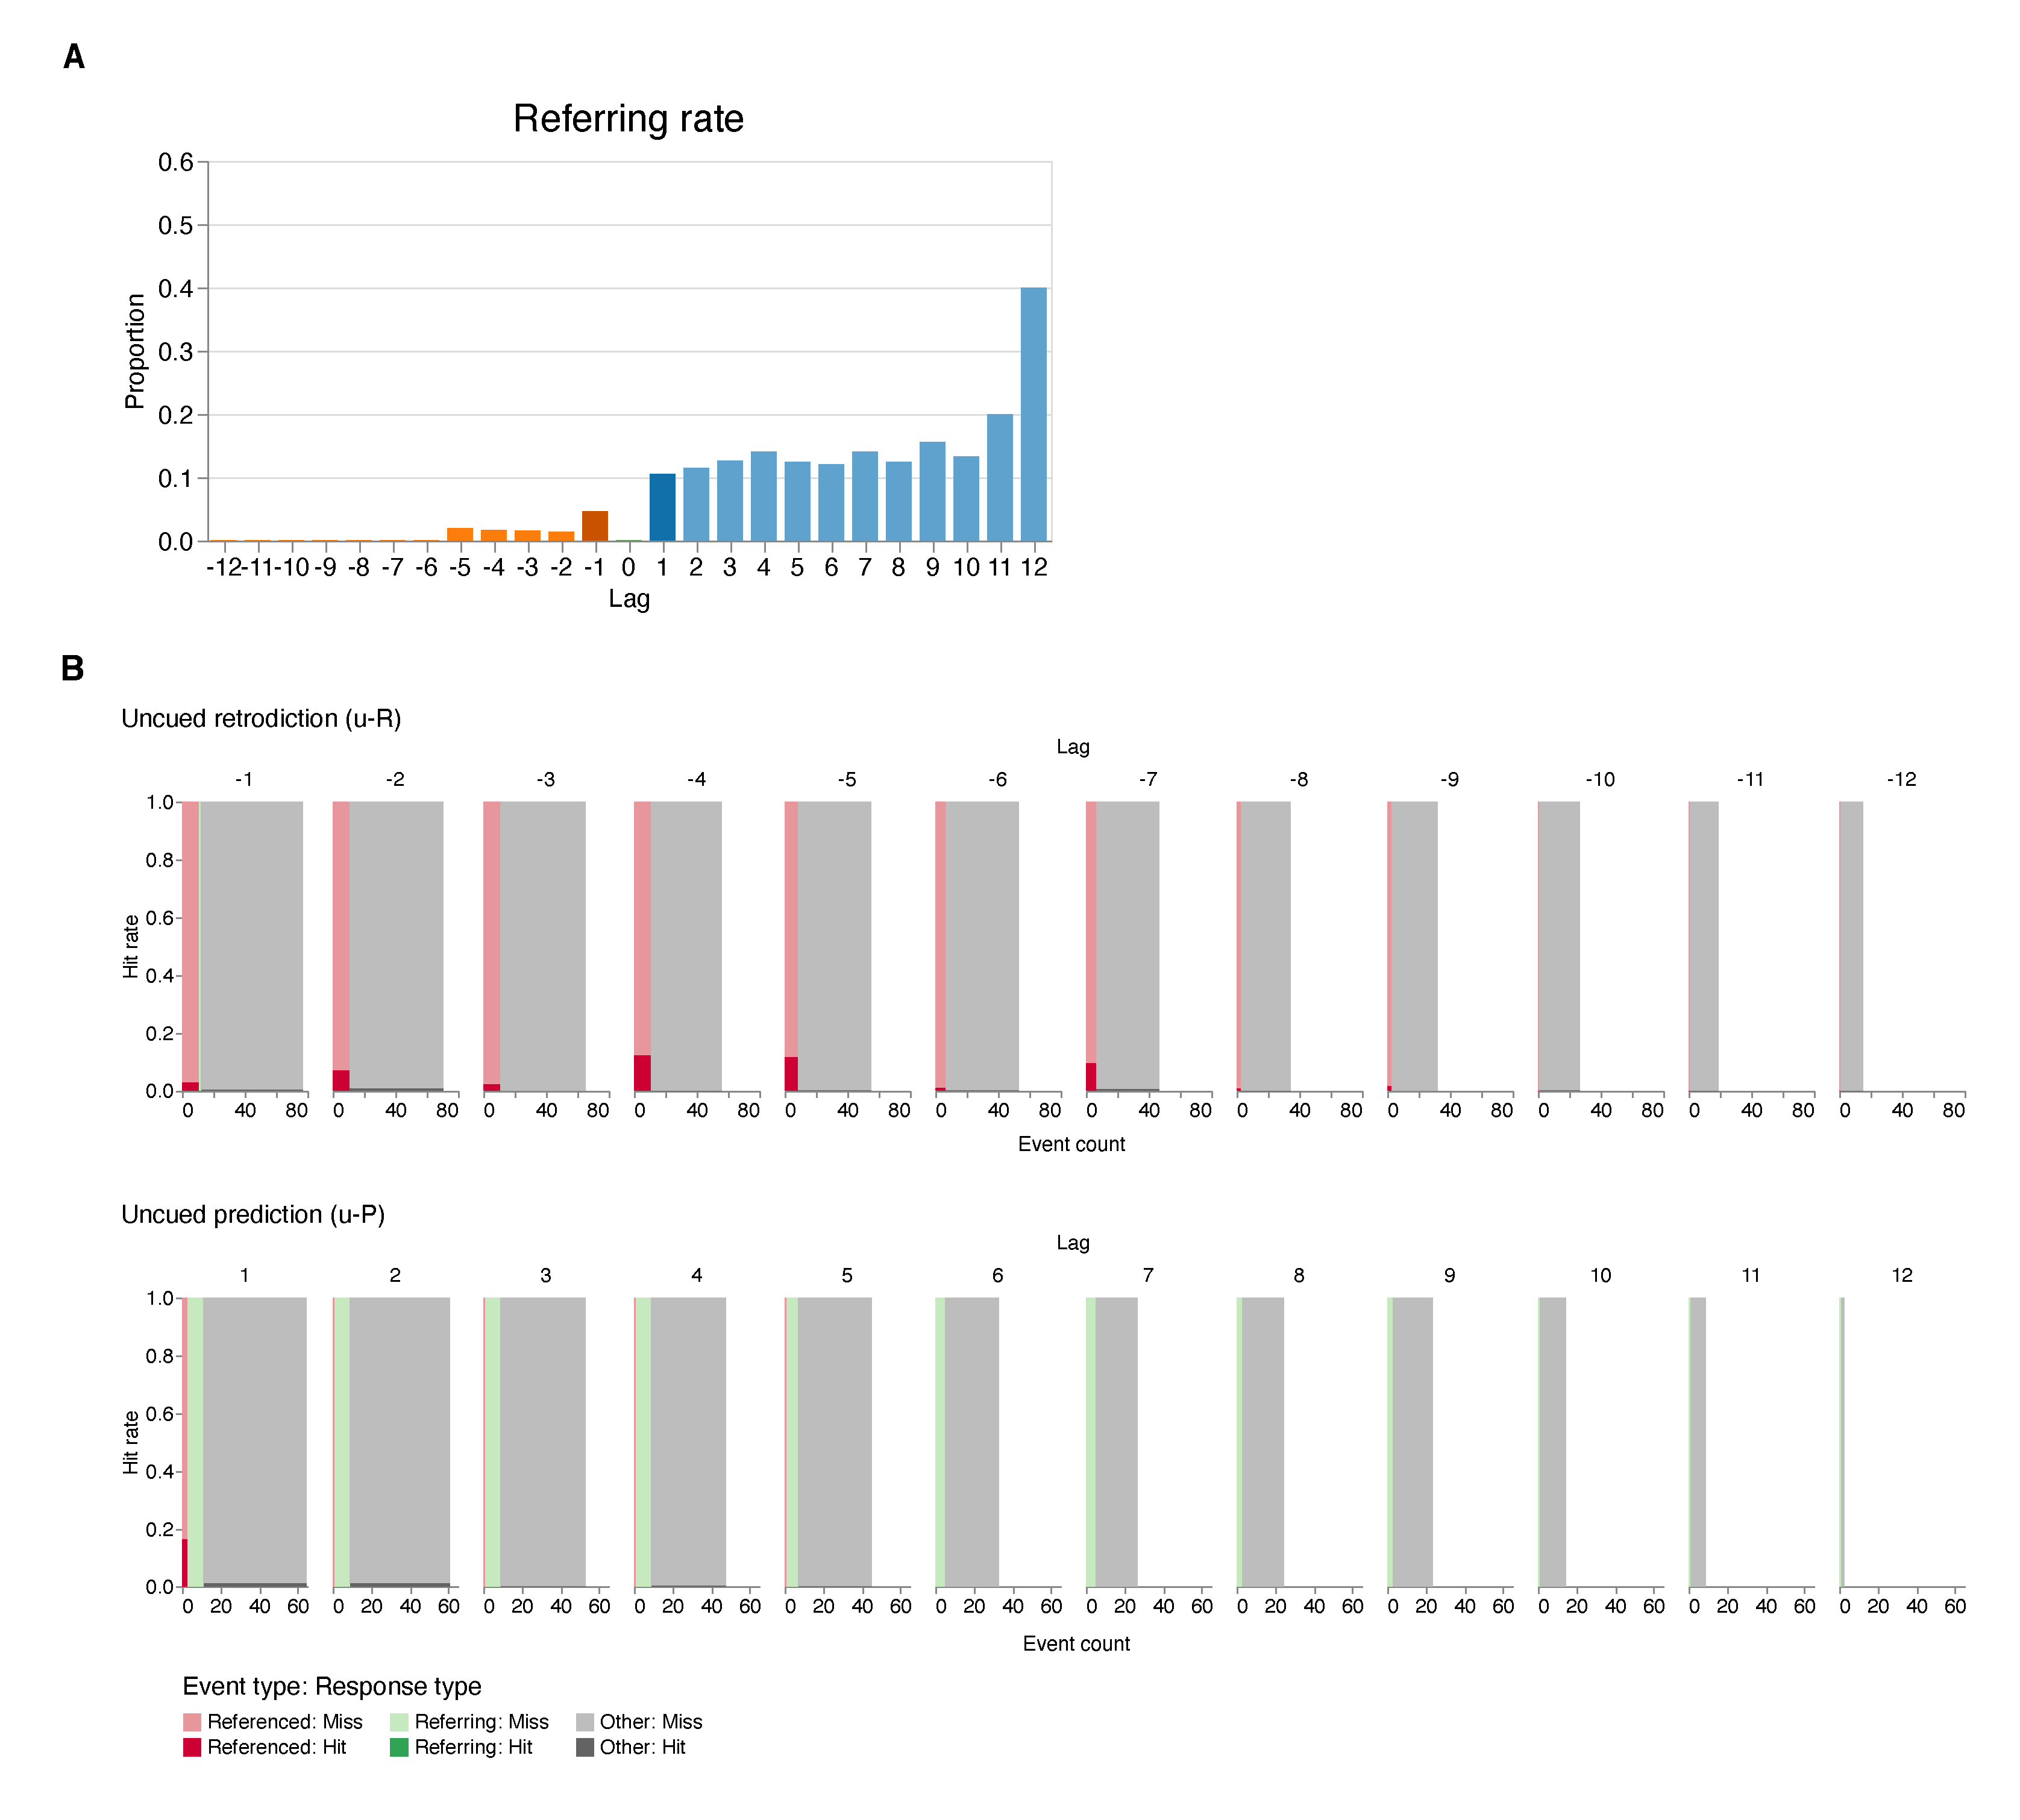
\includegraphics[width=\textwidth]{results5_rep}
      \caption{\textbf{Hit rates for referenced versus referring events (replication experiment).} \textbf{A. Referring rate as a function of lag.} Across all possible just-watched segments (lag 0), the bar heights denote the across-segment mean proportions of events containing references to events in other past or future segments in our replication experiment's stimuli. The bar colors are described in the Figure~\resultTwo~ caption. \textbf{B. Hit rates and counts of referenced, referring, and other events.} As a function of temporal distance to the just-watched segment, the sub-panels display the numbers ($x$-axes) and hit rates ($y$-axes) of referenced (red), referring (green), and other (gray) events that participants hit (darker shading) or missed (lighter shading) in their uncued retrodictions (top sub-panel) and uncued predictions (bottom sub-panel).}
    \label{fig:result5_rep}
\end{figure}

\end{document}